%!TeX program = xelatex
\documentclass[12pt,hyperref,a4paper,UTF8]{ctexart}
\usepackage{ZJUTReport}
\usepackage{listings}
\usepackage{xcolor}

\usepackage{setspace}
\setstretch{1.5} % 设置全局行距为1.5倍

\usepackage{enumitem} % 载入enumitem包以便自定义列表环境
\setlist[itemize]{itemsep=0pt, parsep=0pt} % 设置itemize环境的项目间距和段落间距

\setmainfont{Times New Roman} % 英文正文为Times New Roman

%封面页设置
{   
    %标题
    \title{ 
        \vspace{1cm}
        \heiti \Huge \textbf{{XXXX课程报告}} \par
        \vspace{1cm} 
        \heiti \Large {\underline{XXXXXX进展调研}}    
        \vspace{3cm}
    }

    \author{
        \vspace{0.5cm}
        \kaishu\Large 学院\ \dlmu[9cm]{计算机学院} \\ %学院
        \vspace{0.5cm}
        \kaishu\Large 专业\ \dlmu[9cm]{计算机科学与技术} \\ %班级
        \vspace{0.5cm}
        \kaishu\Large 学号\ \dlmu[9cm]{2023XXXXXX} \qquad  \\ %学号
        \vspace{0.5cm}
        \kaishu\Large 姓名\ \dlmu[9cm]{XXX} \qquad \\ %姓名 
    }
        
    \date{\today} % 默认为今天的日期,可以注释掉不显示日期
}
%%------------------------document环境开始------------------------%%
\begin{document}

%%-----------------------封面--------------------%%
\cover
\thispagestyle{empty} % 首页不显示页码
%%------------------摘要-------------%%
\newpage
\begin{abstract}

在此填写摘要内容

\end{abstract}

\thispagestyle{empty} % 首页不显示页码

%%--------------------------目录页------------------------%%
\newpage
\tableofcontents
% \thispagestyle{empty} % 目录不显示页码

%%------------------------正文页从这里开始-------------------%
\newpage
\setcounter{page}{1} % 让页码从正文开始编号

%%可选择这里也放一个标题
%\begin{center}
%    \title{ \Huge \textbf{{标题}}}
%\end{center}

\section{模板说明}
本模板主要适用于一些课程的平时论文以及期末论文,默认页边距为2.54cm和3.18cm,中文宋体,英文Times New Roman,字号为12pt(小四)。

编译方式:\verb|xelatex -> bibtex -> xelatex*2|


默认模板文件由以下四部分组成:
\begin{itemize}
    \item \texttt{main.tex} 主文件
    \item \texttt{reference.bib} 参考文献,使用bibtex
    \item \texttt{ZJUTReport.sty} 文档格式控制,包括一些基础的设置,如页眉、标题、学院、学号、姓名等
    \item \texttt{figures} 放置图片的文件夹
\end{itemize}

第一次使用时需前往\texttt{ZJUTReportReport.sty} 对标题、姓名、学号、页眉等进行设置,设置完后即可一劳永逸,封面LOGO亦可替换。

默认带有封面页,页码从正文开始。

\section{一些插入功能}
\subsection{插入公式}
行内公式$v-\varepsilon+\phi=2$。

插入行间公式如\autoref{Euler}:
\begin{equation}
    v-\varepsilon+\phi=2
    \label{Euler}
\end{equation}

\subsection{插入图片}
学校图书馆如\autoref{Library}所示,注意这里使用了\verb|~\autoref{}|命令,也就是会自动生成“图”“式”等前缀,无需手动输入。

\begin{figure}[!htbp]
    \centering
    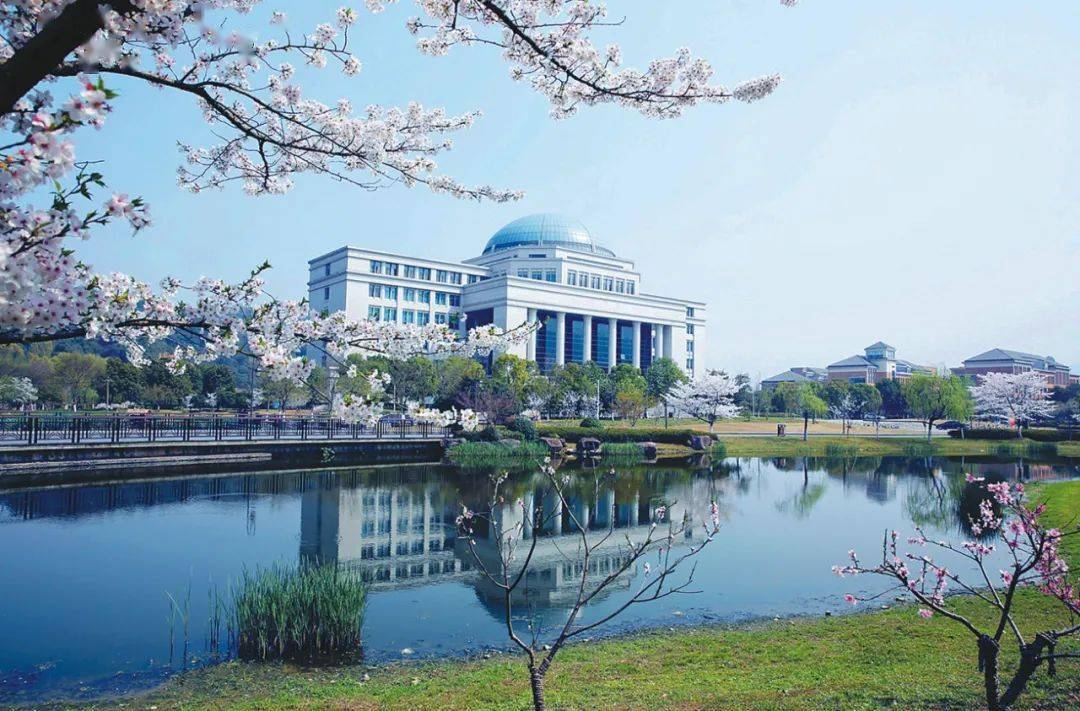
\includegraphics[width =.9\textwidth]{figures/zjut_library.jpeg}
    \caption{浙江公园大学图书馆}
    \label{Library}
\end{figure}

插入上面图片的代码:

\begin{verbatim}
\begin{figure}[!htbp]
    \centering
    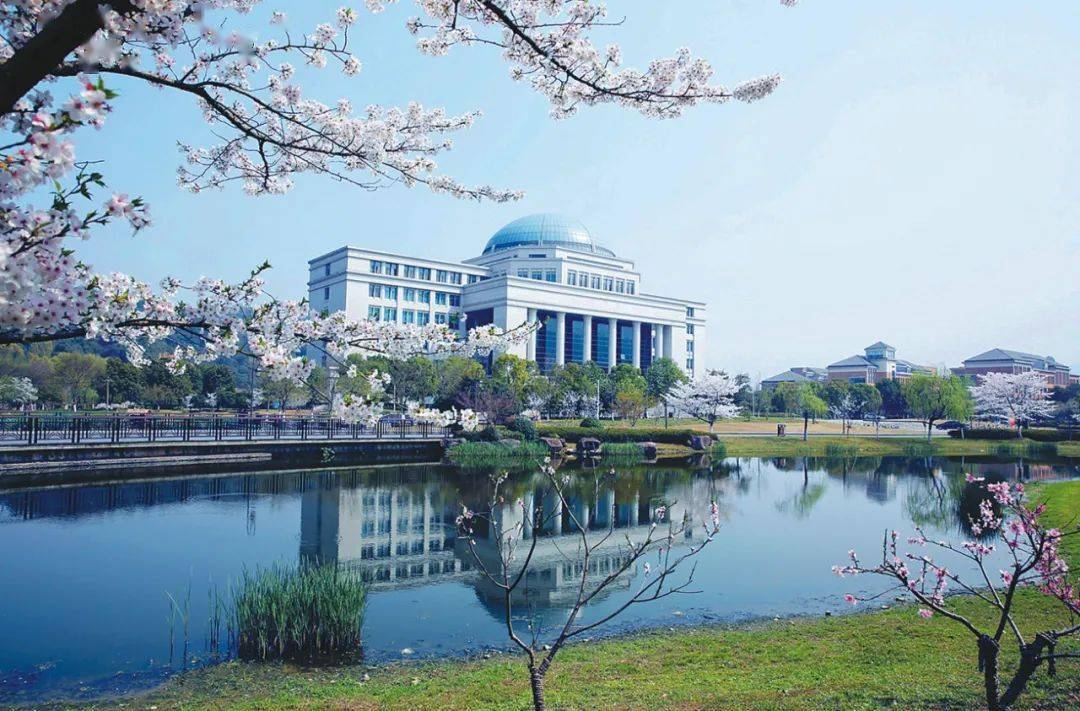
\includegraphics[width =.9\textwidth]{figures/zjut_library.jpeg}
    \caption{浙江公园大学图书馆}
    \label{ZJUT}
\end{figure}
\end{verbatim}

\subsection{插入文本框}
本模板定义了一个圆角灰底的文本框,使用简化命令\verb|\tbox{}|即可,如果你不喜欢,可以前往 \texttt{ZJUTReport.sty}对其进行修改。

\tbox{
    这是一个圆角灰底的文本框
}

\subsection{插入表格}
本模板文件如表~\ref{doc} 所示。
\begin{table}[!htbp]
    \centering
    \begin{tabular}{l  | l}
    \hline
        文件名 & 说明 \\
        \hline
        \texttt{main.tex}  & 主文件 \\
        \texttt{reference.bib} & 参考文献 \\
        \texttt{BUAAReport.sty}  & 文档格式控制\\
        \texttt{figures}  & 图片文件夹 \\
        \hline
    \end{tabular}
    \caption{本模板文件组成}
    \label{doc}
\end{table}

%\section{定理环境}
%\begin{Theorem}
%\end{Theorem}
%
%\begin{Lemma}
%\end{Lemma}
%
%\begin{Corollary}
%\end{Corollary}
%
%\begin{Proposition}
%\end{Proposition}
%
%\begin{Definition}
%\end{Definition}
%
%\begin{Example}
%\end{Example}
%
%\begin{proof}
%\end{proof}

\subsection{插入高亮代码块}
利用\verb|lstlisting| 配置
\begin{lstlisting}[style=CPP, title="c++代码"]
#include <iostream>
#include <array>
int main()
{
    constexpr int MAX = 100;
    std::array<int, MAX> arr;
}  
\end{lstlisting}

\begin{lstlisting}[style=Java, title="Java代码"]
public void addAdvertisement(String company, String ad_Category, String ad_Type, String ad_Price)
{
    int price = Integer.parseInt(ad_Price);
    ad = new Advertisement(company, ad_Category, ad_Type, price);
    adList.add(index, ad);
    index++;
    anDM = getDefaultDirectoryManager();
    ActorTuple tuple = new ActorTuple(getActorName(), "advertiser",
    company, ad_Category, ad_Type, price, index-1);
    send(anDM, "register", tuple);
}
\end{lstlisting}

\begin{lstlisting}[style=Python, title="Python代码"]                
import random
import collections
Card = collections.namedtuple('Card', ['rank', 'suit'])

class FrenchDesk:
    ranks = [str(n) for n in range(2, 11)] + list('JQKA')
    suits = 'spades diamonds clubs hearts'.split()
    
    def __init__(self):
        self._cards = [Card(rank, suit) for rank in self.ranks for suit in self.suits]
        
    def __len__(self):
        return len(self._cards)
        
    def __getitem__(self, position):
        return self._cards[position]
desk = FrenchDesk()
\end{lstlisting}

\subsection{插入参考文献}
直接使用\verb|\cite{}|即可\cite{DBLP:conf/nips/VaswaniSPUJGKP17}。

例如:


   \textit{ 此处引用了文献\cite{0Isaac}。此处引用了文献\cite{2016The}}


引用过的文献会自动出现在参考文献中。

\section{写在最后}
\subsection{发布地址}
\begin{itemize}
    \item Github: \url{https://github.com/ohhhyeahhh/ZJUT_Report_LaTeX_Template}
\end{itemize}


%%----------- 参考文献 -------------------%%
%在reference.bib文件中填写参考文献,此处自动生成

\reference


\end{document}